\documentclass[fontsize=11pt]{article}
\usepackage{amsmath}
\usepackage[utf8]{inputenc}
\usepackage[margin=0.75in]{geometry}
\usepackage[natbibapa]{apacite}
\usepackage{graphicx}
\usepackage{hyperref}


\title{CSC111 Project Proposal:\\\textbf{Animmend - An interactive anime recommendation system}}
\author{
  Ching Chang\\
  \and
  Letian Cheng\\
  \and
  Arkaprava Choudhury\\
  \and
  Hanrui Fan
}
\date{Monday, March 15, 2021}

\begin{document}
\maketitle

\section*{Problem Description and Research Question}
\begin{enumerate}
    \item \textbf{Overview of Background}
    
    \quad Anime is a genre of film and television animation that originated in Japan. Its wide range of storyline and unique art style has attracted over 20 millions audiences since 2018 \citep{Ani18}, and has been significantly scaling in multiple directions in the past 17 years \citep{Ell18}. With over 210 anime published last year in 2020 \citep{wiki21}, there are currently over 17,548 anime in the world \citep{MyA21} — way too many for anyone to pick!
    
    \item \textbf{Problem and Motivation}
    
    \quad This is a problem for both the audience and the producers of the anime who put in their blood and sweat into creating the work, only for it to be buried down in the monstrous pile of anime that are endlessly being published. Although there are anime-recommendation websites and applications out there that recommend users anime they might like based on their watch history, they tend to favour the trend and popular choices. This causes the established studios to self-perpetuate on the top of the pyramid scheme, while the rest that fails to make a good first impression end up at the bottom of the iceberg, forgotten. Much like every other film and television animation, anime is a form of fine arts medium where the authors, artists, and the production team splash their canvas with imagination and creativity. In a field with such freedom and originality, every anime has a meaningful story for someone in the world. Even the most terribly rated anime by the general could be a treasure to the right audience. However, it is difficult finding this so-called “right audience”. Anime with big names speak for themselves, so what the anime community lacks is a bridge between the unheard anime and the audience.
    
    \item \textbf{Our Goal}
    
    \quad To help mitigate this problem, we seek to create \textbf{an application that recommends unpopular anime based on the user’s input anime and relevant themes that they might be interested in.}
\end{enumerate}



\section*{Computational Plan}

\begin{enumerate}
    \item \textbf{Graph Implementation}
    
    \quad \quad Anime is a genre of film and television animation that originated in Japan. Its wide range of storyline and unique art style has attracted over 20 millions audiences since 2018 \citep{Ani18}, and has been significantly scaling in multiple directions in the past 17 years \citep{Ell18}. With over 210 anime published last year in 2020 \citep{wiki21}, there are currently over 17,548 anime in the world \citep{MyA21} — way too many for anyone to pick!
    
    \item \textbf{Problem and Motivation}
    
    \quad This is a problem for both the audience and the producers of the anime who put in their blood and sweat into creating the work, only for it to be buried down in the monstrous pile of anime that are endlessly being published. Although there are anime-recommendation websites and applications out there that recommend users anime they might like based on their watch history, they tend to favour the trend and popular choices. This causes the established studios to self-perpetuate on the top of the pyramid scheme, while the rest that fails to make a good first impression end up at the bottom of the iceberg, forgotten. Much like every other film and television animation, anime is a form of fine arts medium where the authors, artists, and the production team splash their canvas with imagination and creativity. In a field with such freedom and originality, every anime has a meaningful story for someone in the world. Even the most terribly rated anime by the general could be a treasure to the right audience. However, it is difficult finding this so-called “right audience”. Anime with big names speak for themselves, so what the anime community lacks is a bridge between the unheard anime and the audience.
    
    \item \textbf{Our Goal}
    
    \quad To help mitigate this problem, we seek to create \textbf{an application that recommends unpopular anime based on the user’s input anime and relevant themes that they might be interested in.}
\end{enumerate}



\section*{Computational Plan}

\begin{enumerate}
    \item \textbf{Graph Implementation}
    
    \quad The recommendation model will be initialized using more than 30,000 anime data taken from the Manami database. Each anime from the Manami database contains one or more “tags” that label the sub-genre, topic, and theme. We will create a function that reads through all 31,166 animes from the Manami database and determines 20 related anime for each anime based on the tags and similarity. Each anime and their related anime, as well as their corresponding tags, will be saved into a \textbf{JSON} file to be processed prior to the production stage. This shortens the time needed to construct the graph for users.
    
    \quad We use a graph structure to represent the collection of anime in our database. Each vertex in the graph represents a single anime. We create a custom class “Anime” that contains a string of an anime’s name, and a list of values representing the relevance of each “tag” for that particular anime (the relevance are ordered in a way such that all they represent the tags in a certain order defined by us). The similarity of the anime with other anime can be seen as the dot product of their ‘tag vectors’ which can be calculated using \textbf{NumPy}’s dot product function, partly inspired by the vector space model used in search engines \citep{vspace}. The weights are normalized for each anime, and all relevant tags for the anime are weighted equally. As users provide feedback on the recommendations, the program automatically re-adjusts the weighting of each tag using vector normalization, and recomputes the similarity with other anime. An anime’s neighbours are those vertices whose similarities with the dot product greater than a predefined threshold. To simplify the process of visualization, a vertex is restricted to a maximum of twenty neighbours; this implementation keeps users' convenience in mind, as one would seldom be interested in scrolling past more than twenty recommendations. We can also add new anime to the graph whenever new anime are included in the Manami database; however, as such an operation is $\Theta(n^2)$ (where $n$ is the number of existing vertices), it is not realistic to include in the user interface.
    
    \item \textbf{Data Example}
    
    \href{https://gist.github.com/RealFakeAccount/cf34244d17039e78512428a1cf51d95f}{Data Example saved on GitHub} \citep{manami}
    
    \item \textbf{Visualization and Interactions}
    
    \begin{center}
        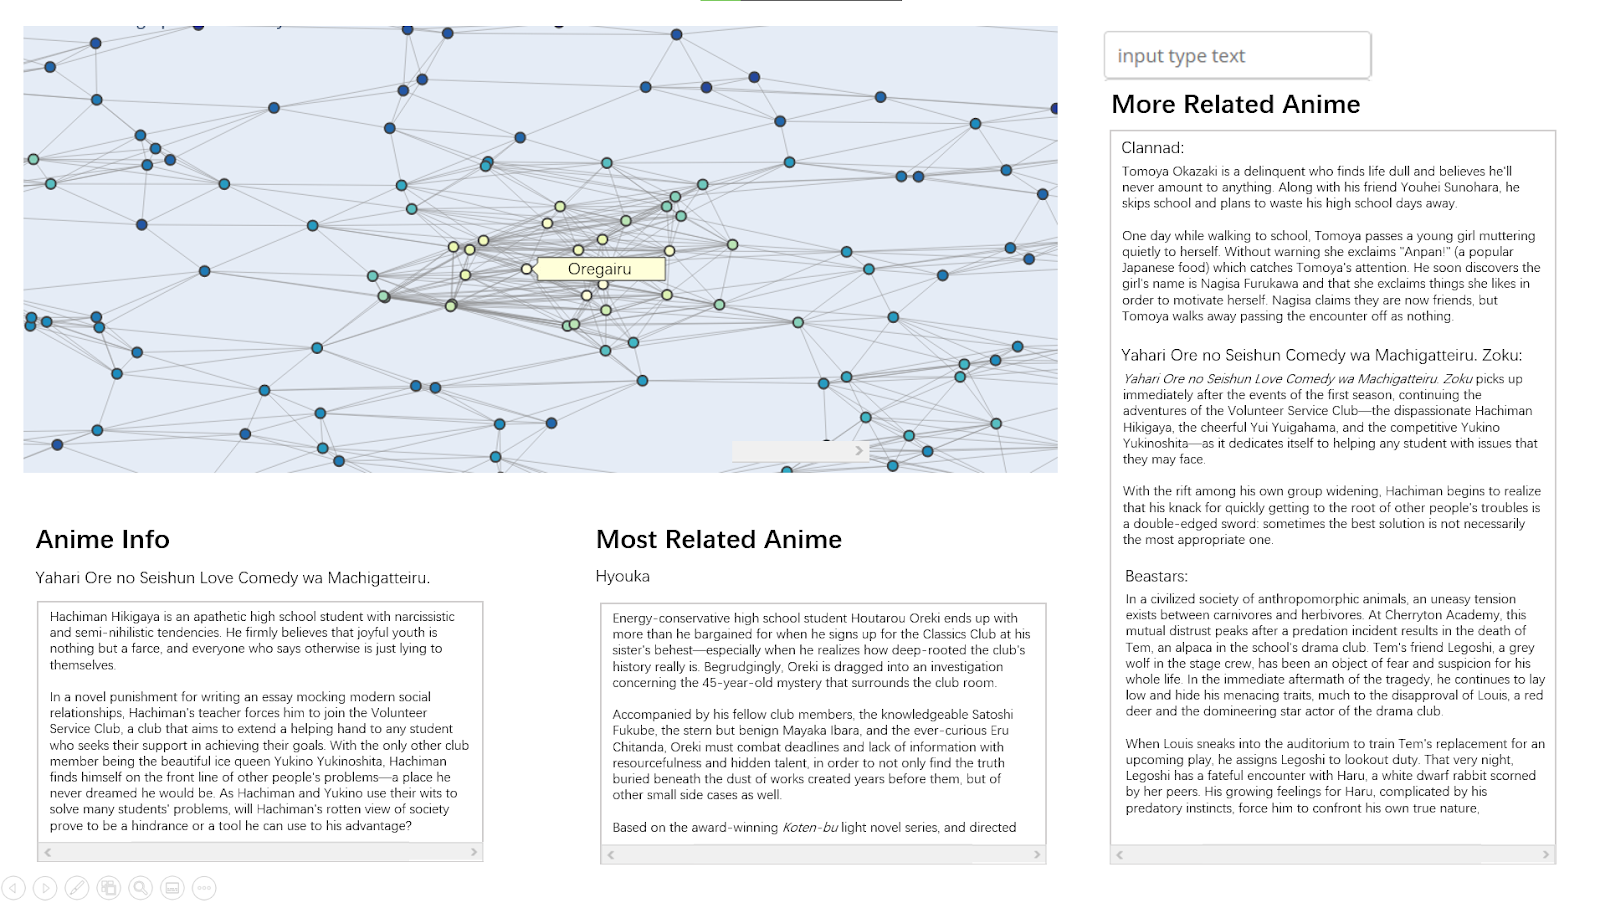
\includegraphics[scale=.2]{Interface Example.png}
        
        Interface Example
    \end{center}
    
    \quad There will be an input box where the user can input an anime that they would like to search. Our program would parse the existing \textbf{JSON} file that we saved earlier and display all anime connected to the one that the user input, for up to depth 3. The user will be able to click on the nodes of the graph to see an overview of the recommended anime, as well as a ranking of 20 anime ranked by similarity. Each overview of the recommendation comes with a “like” and “dislike” for the user to provide feedback on the quality of our recommendation which will be used to automatically adjust the weighting of the tags, according to the tags that the recommendations correspond to.
    
    \item \textbf{Technical Requirement}
    
    \quad \textbf{JSON} is a format that provides lightweight data interchange originated from \textbf{JavaScript} \citep{JSON21}. We import the Python library version of \textbf{JSON} to exchange and store all the animation data from the Manami database \citep{Pyjson}. 

    \quad \textbf{Pandas} is a Python library written for data manipulation and analysis \citep{Pan21}. Also, in order to pass data to create visualization. We use \textbf{pandas} for \textbf{JSON} reading and provide data to graph the relationship between nodes.
    
    \quad \textbf{NumPy} is a Python library that assists scientific calculation \citep{Pynpy}. In particular, we use \textbf{NumPy} to do vector dot products and normalizations, to update similarity (our most important feature) between nodes.
    
    \quad \textbf{Plotly} is a Python open-sourced library that helps to make interactive, publication-quality graphs \citep{plotly}. Specifically, we use \textbf{Plotly} to draw the graph and show the relationship between each node by a web page created by \textbf{Dash}.
    
    \quad \textbf{Dash} is a Python-based open-sourced library written for building web analytic applications based on \textbf{Plotly} \citep{Dash21}. In particular, we use \textbf{Dash} and \textbf{Plotly} to build web pages that interact with users to present new content recommended by our program based on user input and can access our content on any platform.
    
\end{enumerate}

\bibliography{references}
\bibliographystyle{apacite}

\end{document}
